\documentclass[tikz,border=4pt]{standalone}
\usepackage{amsmath}
\begin{document}
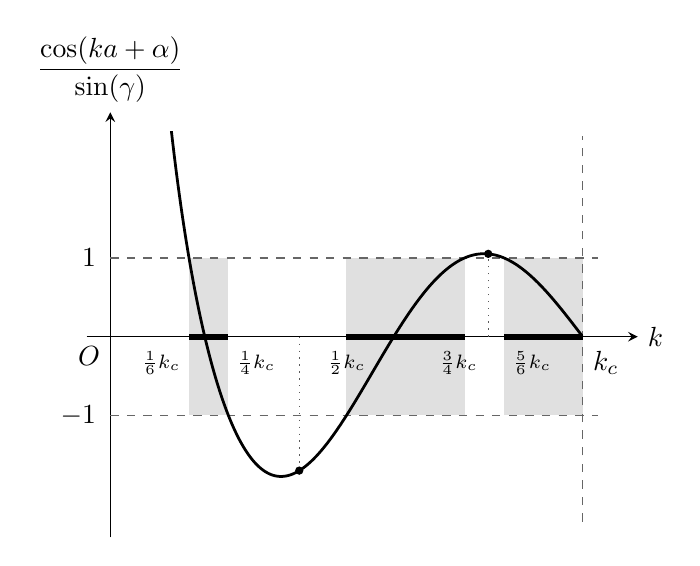
\begin{tikzpicture}[>=stealth, thick, scale=1.0]
  % Plot f(k) = cos((kc*a - c)*u) / sin((pi/2)*u) for u = k/kc in (0, 1)
  % Representative case: kc*a - c = 5*pi/2 (450 deg)
  % Horizontal scale: x = 6.0 * u (so kc is at x = 6.0)
  % Vertical scale: y = 1.0 * f (clipped to [-2.5, 2.7])

  % Allowed band shading along k-axis (|f| <= 1)
  % Band 1: u in [1/6, 1/4] => x in [1.0, 1.5]
  % Band 2: u in [1/2, 3/4] => x in [3.0, 4.5]
  % Band 3: u in [5/6, 1]   => x in [5.0, 6.0]
  \fill[black!12] (1.0, -1.0) rectangle (1.5, 1.0);
  \fill[black!12] (3.0, -1.0) rectangle (4.5, 1.0);
  \fill[black!12] (5.0, -1.0) rectangle (6.0, 1.0);

  % Axes
  \draw[->, line width=0.55pt] (-0.3, 0) -- (6.7, 0) node[right] {$k$};
  \draw[->, line width=0.55pt] (0, -2.55) -- (0, 2.85) node[above] {$\dfrac{\cos(ka+\alpha)}{\sin(\gamma)}$};
  \node[below left] at (0, 0) {$O$};

  % Dashed lines at y = +1, -1 and x = kc
  \draw[dashed, line width=0.5pt, black!60] (0, 1.0) -- (6.2, 1.0);
  \draw[dashed, line width=0.5pt, black!60] (0, -1.0) -- (6.2, -1.0);
  \draw[dashed, line width=0.5pt, black!60] (6.0, -2.35) -- (6.0, 2.55);
  \node[left] at (-0.05, 1.0) {$1$};
  \node[left] at (-0.05, -1.0) {$-1$};
  \node[below right] at (6.0, -0.05) {$k_c$};

  % Highlight allowed bands on k-axis
  \draw[line width=2.2pt] (1.0, 0) -- (1.5, 0);
  \draw[line width=2.2pt] (3.0, 0) -- (4.5, 0);
  \draw[line width=2.2pt] (5.0, 0) -- (6.0, 0);

  % Curve clipped vertically to [-2.4, 2.6]
  \begin{scope}
    \clip (0.01, -2.4) rectangle (6.05, 2.6);
    \draw[line width=1.0pt, domain=0.12:1.0, samples=300]
      plot ({6.0*\x}, {cos(450*\x) / sin(90*\x)});
  \end{scope}

  % Mark Bragg points (ka + alpha = pi, 2pi => u = 2/5, 4/5 => x = 2.4, 4.8)
  % f(2/5) = -1/sin(36) = -1.7013; f(4/5) = 1/sin(72) = 1.0515
  \draw[dotted, line width=0.5pt, black!65] (2.4, 0) -- (2.4, -1.701);
  \fill (2.4, -1.701) circle (1.5pt);
  \draw[dotted, line width=0.5pt, black!65] (4.8, 0) -- (4.8, 1.052);
  \fill (4.8, 1.052) circle (1.5pt);

  % Key tick labels on k-axis
  \node[below left, font=\scriptsize] at (1.02, -0.06) {$\frac{1}{6}k_c$};
  \node[below right, font=\scriptsize] at (1.48, -0.06) {$\frac{1}{4}k_c$};
  \node[below, font=\scriptsize] at (3.0, -0.06) {$\frac{1}{2}k_c$};
  \node[below, font=\scriptsize] at (4.42, -0.06) {$\frac{3}{4}k_c$};
  \node[below right, font=\scriptsize] at (4.98, -0.06) {$\frac{5}{6}k_c$};
\end{tikzpicture}
\end{document}
